\section{Ziel}
    Ziel dieses Versuches ist es die räumliche Zusammensetzung eines Objektes zu bestimmen. Dazu wird die Methodik der Gamma-Tomographie genutzt. Bei dieser werden entlang mehrerer räumlicher
    Achsen des Objekts Absorptionsmessungen mit Gammastrahlung durchgeführt, die in Kombination auf die räumliche Zusammensetzung schließen lassen.   
    
\section{Theoretische Grundlagen}
    \subsection{Gammaquellen}
        %Für die notwendigen Absorptionsmessungen muss zunächst Gammastrahlung erzeugt werden. Gammastrahlung beschreibt Photonen mit einer Energie über \SI{200}{\kilo\electronvolt} und kann auch verschiedenen
        %Wegen entstehen. Hier soll die Entstehung bei radioaktiven Zerfällen betrachtet werden. Explizit werden die $\beta^-$-Zerfälle von \ce{^{137}Cs} und \ce{^{60}Co} betrachtet. Diese Elemente zerfallen 
        %zunächst in angeregte Zustände eines weiteren Elements und gehen dann unter Aussendung eines Photons in dessen Grundzustand über. Wie in Abbildung ... zu sehen, kann \ce{^{137}Cs} nur in einen 
        %angeregten Zustand von \ce{^{137}Ba} zerfallen. Bei dessen Übergang in den Grundzustand $ \ce{^{137}Ba}^* \rightarrow \ce{^{137}Ba} + \gamma$ wird ein Photon der Energie \SI{661.7}{\kilo\electronvolt}
        %ausgesendet. Demnach strahlt eine ein \ce{^{137}Cs} mit einer maximalen Intensität bei der angegebenen Energie von \SI{661.7}{\kilo\electronvolt}.

        Für die notwendigen Absorptionsmessungen muss zunächst Gammastrahlung erzeugt werden. Gammastrahlung beschreibt Photonen mit einer Energie über \SI{200}{\kilo\electronvolt} und kann auf verschiedenen
        Wegen entstehen. Hier soll die Entstehung bei radioaktiven Zerfällen betrachtet werden. Explizit wird der $\beta^-$-Zerfall von \ce{^{137}Cs}, das in diesem Versuch als Gammaquelle dient, betrachtet. 
        %Dieses Element zerfällt teils in einen angeregten Zustand eines weiteren Elements und geht dann unter Aussendung eines Photons in dessen Grundzustand über. 
        Wie in Abbildung \ref{fig:cs_schema} zu sehen, 
        ist für \ce{^{137}Cs} neben dem direkten Übergang in den Grundzustand von \ce{^{137}Ba} mit einer Wahrscheinlichkeit von \SI{6.5}{\percent} der Übergang in einen angeregten Zustand von \ce{^{137}Ba} mit
        einer Wahrscheinlichkeit von \SI{93.5}{\percent} deutlich wahrscheinlicher. Bei dem Übergang aus dem angeregten Zustand in den Grundzustand $ \ce{^{137}Ba}^* \rightarrow \ce{^{137}Ba} + \gamma$ wird ein 
        Photon der Energie \SI{661.7}{\kilo\electronvolt} ausgesendet. Demnach strahlt eine \ce{^{137}Cs}-Quelle mit einer maximalen Intensität bei der angegebenen Energie von \SI{661.7}{\kilo\electronvolt}.

        \FloatBarrier

        \begin{figure}[h]
          \centering
          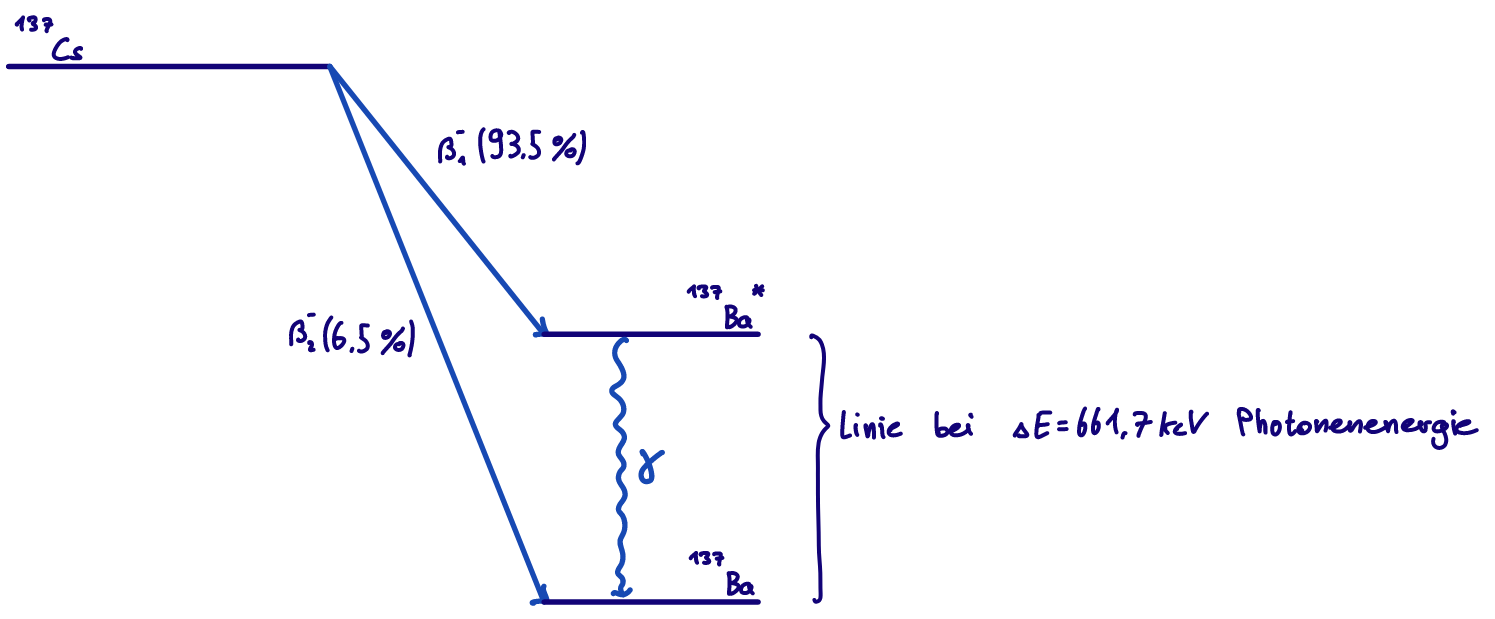
\includegraphics[width = 1\textwidth]{pictures/cs.png}
          \caption{Die möglichen $\beta^-$-Zerfälle von \ce{^{137}Cs} in \ce{^{137}Ba} sowie dessen angeregten Zustand \ce{^{137}Ba}$^*$ und anschließender Übergang in den Grundzustand von \ce{^{137}Ba} unter Aussendung eines Photons. Bearbeitet aus \cite{stolz_radioaktivitat_2003}}
          \label{fig:cs_schema}
        \end{figure}
    
        \FloatBarrier
        
        %Für den in Abbildung ... skizzierten Zerfall von \ce{^{60}Co} sind Übergänge in zwei verschiedene angeregte Zustände von \ce{^{60}Ni} möglich. Der energetisch höhere Zustand liegt bei 
        %\SI{2505.7}{\kilo\electronvolt} und der niedrigere bei \SI{1332.5}{\kilo\electronvolt}. Der energetisch niedrigere Zustand geht direkt in den Grundzustand über und es wird ein Photon mit einer Energie
        %von \SI{1332.5}{\kilo\electronvolt} ausgesendet. Die Relaxation des energetisch höheren Zustands findet in zwei Schritten statt. Zunächst geht dieser Zustand in den niederenergetischen angeregten Zustand 
        %über, wobei ein Photon mit der Energie \SI{1173.2}{\kilo\electronvolt} ausgesendet wird. Anschließend geht es in den Grundzustand des \ce{^{60}Ni} über. Aufgrund der zwei angeregten Endzustände des 
        %$\beta^-$-Zerfalls strahlt eine \ce{^{60}Co}-Quzelle mit zwei charakteristischen Energien.
%
        %\FloatBarrier
%
        %\begin{figure}[h]
        %  \centering
        %  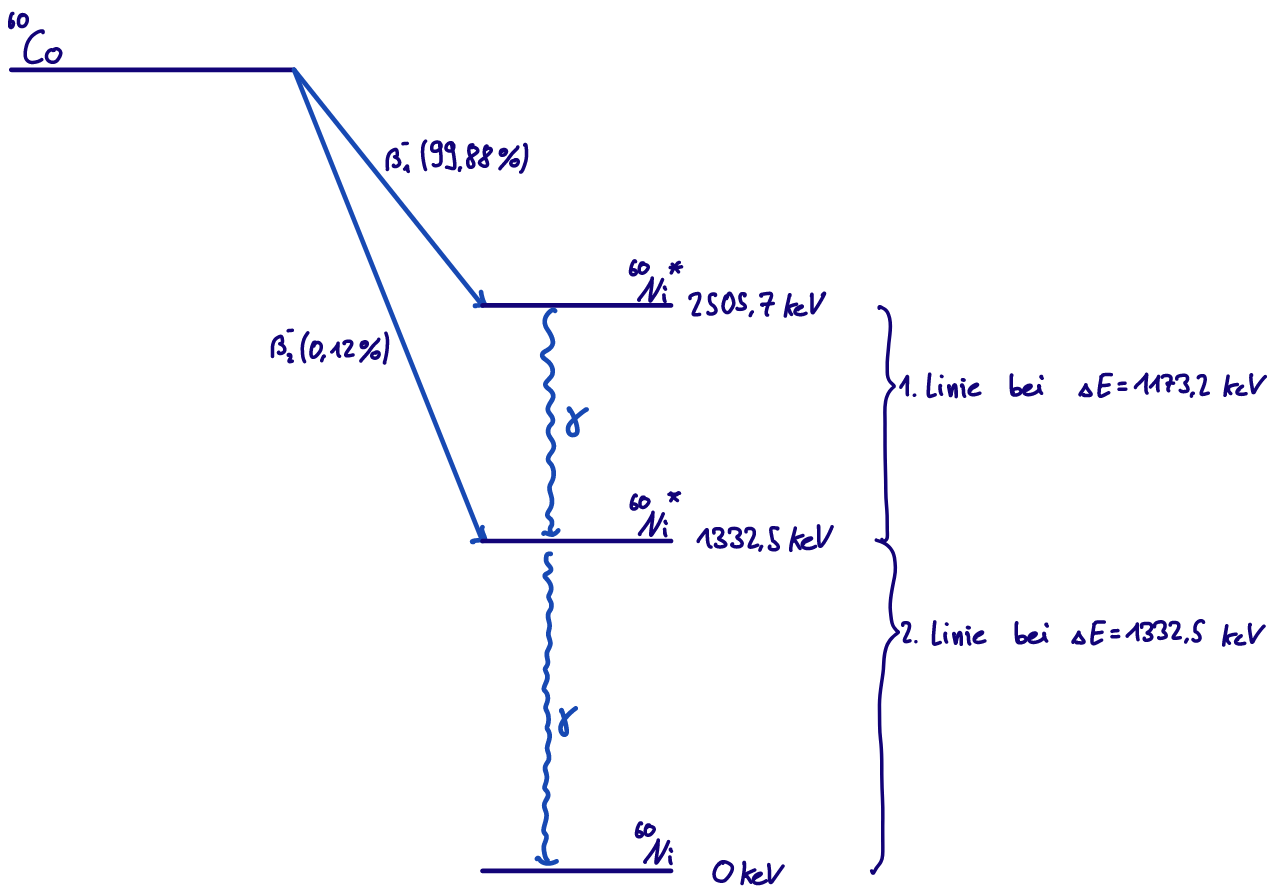
\includegraphics[width = 1\textwidth]{pictures/co.png}
        %  \caption{Die möglichen $\beta^-$-Zerfälle von \ce{^{60}Co} in die angeregten Zustände von \ce{^{60}Ni} und anschließende Übergänge in den Grundzustand von \ce{^{60}Ba} unter Aussendung zwei Photonen verschiedener Energien. Bearbeitet aus \cite{stolz_radioaktivitat_2003}}
        %  \label{fig:co_schema}
        %\end{figure}
    %
        %\FloatBarrier

      \subsection{Absorption von Photonen}
        Die Absorption von Photonen wird über die Änderung der Intensität $I$ einer Strahlungsquelle über das \textbf{Lambert-Beerśche-Gesetz} beschrieben

        \begin{equation}
          I(x) = I_0 \exp\left(-\mu x\right),
        \label{eqn:absorptionsgesetz}
        \end{equation}

        das die Intensität $I$ in einer Entfernung $x$ von einem Ausgangspunkt mit der Ausgangsintensität $I_0$ in Abhängigkeit der Entfernung und des Absorptionskoefizientens $\mu$ des Ausbreitungsmediums 
        angibt. Der gesamte Absorptionskoefizient $\mu$ ist die Summe der Absorptionskoefizienten vieler Prozesse
        
        \begin{equation*}
          \mu = \mu_{PE} + \mu_{CS} + \mu_{PP} + \mu_{RS},
        \end{equation*}

        wie der Photoemission (PE), der Compton-Streuung (CS), der Paar-Produktion (PP) und der Rayleigh-Streuung (RS). Der gesamte Absorptionskoefizient $\mu$ ist zum einen von der Photonenenergie $E$ und 
        vom Ausbreitungsmedium abhängig. In Abbildung \ref{fig:absorptionskoeffizient} ist der energieabhängige Verlauf des gesamten Absorptionskoefizientens sowie der der hauptsächlich beitragenden 
        Absorptionskoefizienten der Paar-Produktion, Photoemission und Compton-Streuung für Germanium dargestellt. 

        \FloatBarrier

        \begin{figure}[h]
          \centering
          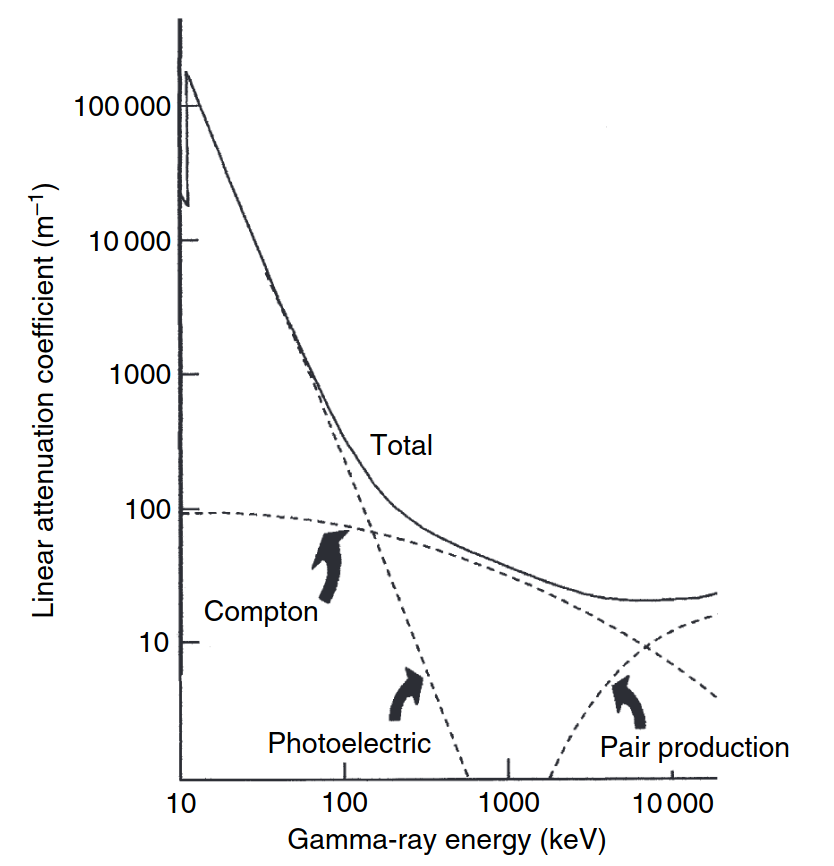
\includegraphics[width = 0.6\textwidth]{pictures/absorptionskoeffizient.png}
          \caption{Der energieabhängige Verlauf des Absorptionskoefizientens von Germanium und dessen Bestandteilen der einzelnen Prozesse (PP, PE, CS).Entnommen aus \cite{gilmore_practical_2008}}
          \label{fig:absorptionskoeffizient}
        \end{figure}

        Exemplarisch wird die Absorption von Gammastrahlung aus einer \ce{^{137}Cs}-Quelle mit der Aktivität $A_{\text{Quelle}} = \SI{18}{\mega\becquerel}$ betrachtet, die $D=\SI{3}{\centi\metre}$ durch einen 
        Bleiblock und $L-D = \SI{29}{\centi\metre}$ durch Luft zurücklegt. Die am Detektor theoretisch zu messende Aktivität erigbt sich zu

        \begin{equation*}
          A_{\text{Detektor}} = A_{\text{Quelle}} \cdot \exp\left(-\mu_{\text{Luft}}\left(L-D\right) - \mu_{\text{Pb}}D\right) \approx \SI{422536}{\per\second} \approx \SI{0.42}{\mega\becquerel}.
        \end{equation*}
    
        \FloatBarrier

      \newpage
      \subsection{Intensitätsmessung}
        Um die Intensität der Strahlung in Abhängigkeit der Energie zu messen, wird von einem \textbf{Szintillationsdetektor} in Kombination mit einem \textbf{Diskrimantor} und einem 
        \textbf{Vielkanal-Analysator} Gebrauch gemacht.

        \subsubsection*{Szintillationsdetektor}
          Das Konzept von Szintillatoren beruht darauf, dass einfallende Strahlung hoher Energie Atome des Szintillationsmediums entweder ionisiert oder anregt und 
          diese beim Relaxieren optische Photonen freisetzen. Die Menge an freigesetzten Photonen hängt dabei von der Energie der einfallenden Strahlung ab. Die optischen Photonen des Relaxationsprozesses 
          werden anschließend von Photomultipliern detektiert. %Grundlegend wird zwischen organischen und anorganischen Szintillatoren unterschieden.
        \newpage
        \subsubsection*{Diskriminatoren}
          Um nur optische Photonen aus dem Szintillationsdetektor zu detektieren wird ein Diskrimantor eingesetzt. Dieser gibt erst ab einem einen Schwellwert übersteigenden Eingangssignal ein Ausgangssignal 
          aus. So kann verhindert werden, dass bereits ein einzelnes spontan emmitiertes Photon einen Ausgangsimpuls am Photomultiplier hervorruft, der fälschlicherweise auf ein optisches Photon des 
          Szintillationsdetektors zurückgeführt werden würde.

        \subsubsection*{Vielkanal-Analysator}
          Aus dem Photomultiplier erreichen den Vielkanal-Analysator elektrische Signale, deren Stärke proportional zur Energie der Strahlung, die ein Szintillationselektron anregt, angenommen werden kann. 
          Der Vielkanal-Analysator besitzt nun einen digitalen Speicher, der für die verschiedenen Impulstärken verschiedene Speicherplätze besitzt. Die Impulsstärken und zugehörigen Speicherplätze sind
          Photonenenergien der die Szintillationselektronen anregenden Strahlung zugeordnet. Durch die Einsortierung der eingehenden Impulse in die verschiedenen Speicherplätze, kann so 
          ein Histogramm erstellt werden, dass die energieabhängige Intensität der auf den Detektor treffenden Intensität darstellt.

        \subsubsection*{Repräsentative Messung}
          Die Intensitätsmessung gibt Counts aus, die der Anzahl an detektierten Photonen entspricht. Damit die Messung als repräsentativ angesehen werden kann, wird eine statistische Unsicherheit von 
          mindestens \SI{3}{\percent} gefordert. Unter der Annahme, dass die Zählrate poisson-verteilt ist, kann somit eine minimal benötigte Zahl an Counts $N$ berechnet werden

          \begin{equation*}
            \frac{\Delta N}{N} = \frac{\sqrt{N}}{N} \le 0,03 \qquad \rightarrow \qquad N \gtrsim 1111,
          \end{equation*}

          die für die geforderte statistische Unsicherheit erforderlich ist.

      \newpage
      \subsection{Tomographie}
          In diesem Versuch soll die Zusammensetzung von neun Würfeln innerhalb einer 3x3-Würfelebene bestimmt werden. Dazu wird der Würfel aus verschiedenen Richtungen bestrahlt und die transmittierte 
          Intensität gemessen. In eine Richtung i ergibt sich diese zu

          \begin{equation}
            I_{\text{i}} = I_0 \cdot \exp\left(-\sum_{\text{j}} \mu_{\text{j}} d_{\text{j}} \right).
            \label{eqn:I_i}
          \end{equation}

          wobei $I_0$ die Grundintensität beschreibt. Die Summe innerhalb der Exponentialfunktion läuft über alle Materialien j, die die Gammastrahlung durchläuft. $\mu_{\text{j}}$ beschreibt den 
          Absorptionskoefizienten des entsprechenden Materials und $d_{\text{j}}$, die Distanz, die durch jenes Material zurückgelegt wird. Um Rückschlüsse auf die Zusammensetzung des Würfels ziehen zu können,
          wird der natürliche Logarithmus von Gleichung \ref{eqn:I_i} gebildet
          
          \begin{equation}
            -\sum_{\text{j}} \mu_{\text{j}} d_{\text{j}} = \ln\left(\frac{I_{\text{j}}}{I_0}\right) \equiv \tilde{I_{\text{j}}}
          \end{equation}

          und zur einfacheren Betrachtung des Gleichungssystems für alle vermessenen Strahlrichtungen als Matrixgleichung formuliert

          \begin{equation}
            -\underline{\underline{A}} \vec{\mu} = \vec{\tilde{I}}.
            \label{eqn:I_matrix}
          \end{equation}

          Die in diesem Versuch zu vermessenden zwölf Bestrahlungsrichtungen sind in Abbildung \ref{fig:Richtungen} dargestellt.

          \FloatBarrier

          \begin{figure}[h]
            \centering
            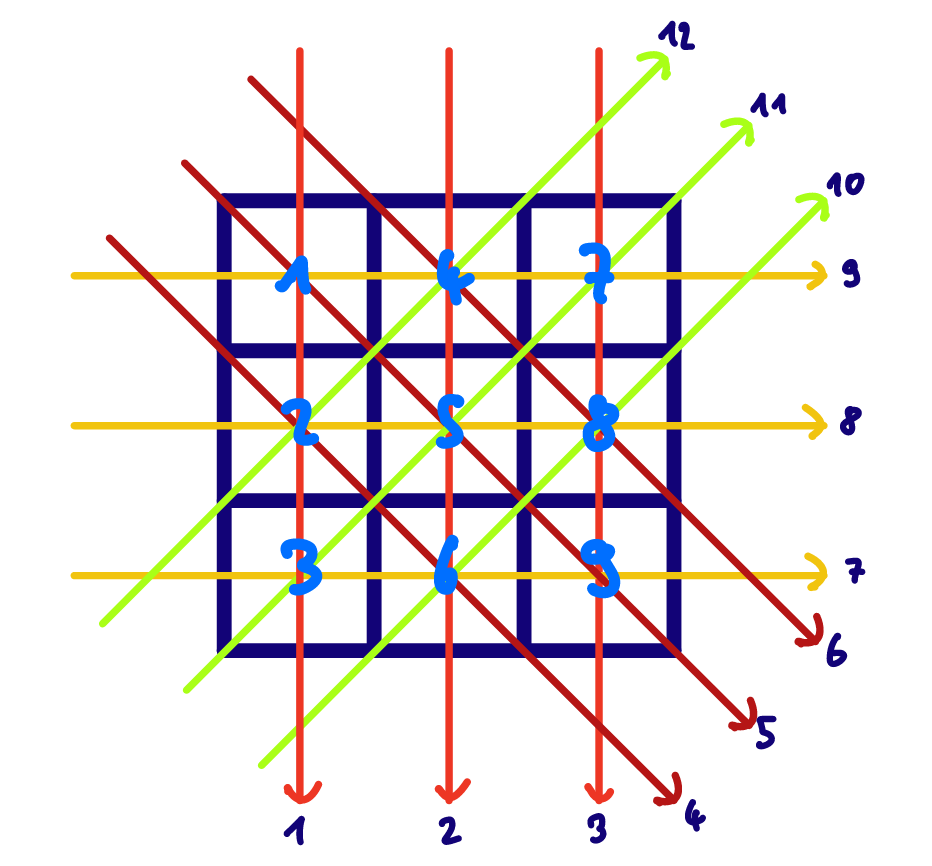
\includegraphics[width = 0.6\textwidth]{pictures/richtungen.png}
            \caption{Die aus neun gleichförmigen Würfeln bestehende Würfelebene sowie die zwölf vermessenen Bestrahlungsrichtungen.}
            \label{fig:Richtungen}
          \end{figure}
      
          \FloatBarrier


          Unter der Annahme, dass die Würfel möglicherweise alle aus einem anderen Material sind und alle die Kantenlänge $d$ besitzen, lässt sich Gleichung \ref{eqn:I_matrix} in diesem Fall explizit 
          aufstellen:
        
          \begin{equation}
            d \cdot
            \begin{pmatrix}
              1 & 1 & 1 & 0 & 0 & 0 & 0 & 0 & 0 \\
              0 & 0 & 0 & 1 & 1 & 1 & 0 & 0 & 0 \\
              0 & 0 & 0 & 0 & 0 & 0 & 1 & 1 & 1 \\
              0 & \sqrt{2} & 0 & 0 & 0 & \sqrt{2} & 0 & 0 & 0 \\
              \sqrt{2} & 0 & 0 & 0 & \sqrt{2} & 0 & 0 & 0 & \sqrt{2} \\
              0 & 0 & 0 & \sqrt{2} & 0 & 0 & 0 & \sqrt{2} & 0 \\
              0 & 0 & 1 & 0 & 0 & 1 & 0 & 0 & 1 \\
              0 & 1 & 0 & 0 & 1 & 0 & 0 & 1 & 0 \\
              1 & 0 & 0 & 1 & 0 & 0 & 1 & 0 & 0 \\
              0 & 0 & 0 & 0 & 0 & \sqrt{2} & 0 & \sqrt{2} & 0 \\
              0 & 0 & \sqrt{2} & 0 & \sqrt{2} & 0 & \sqrt{2} & 0 & 0 \\
              0 & \sqrt{2} & 0 & \sqrt{2} & 0 & 0 & 0 & 0 & 0 
            \end{pmatrix}
            \cdot
            \begin{pmatrix}
              \mu_1 \\
              \mu_2 \\
              \mu_3 \\
              \mu_4 \\
              \mu_5 \\
              \mu_6 \\
              \mu_7 \\
              \mu_8 \\
              \mu_9 
            \end{pmatrix}
            =
            \begin{pmatrix}
              I_1 \\
              I_2 \\
              I_3 \\
              I_4 \\
              I_5 \\
              I_6 \\
              I_7 \\
              I_8 \\
              I_9 \\
              I_10 \\
              I_11 \\
              I_12 \\
            \end{pmatrix}
            \label{unsere_matrix}
          \end{equation}

           

